\documentclass{article}

\usepackage{graphicx}
\usepackage{fancyhdr}
\usepackage[sorting=none]{biblatex}
\usepackage[margin=1in]{geometry}
\usepackage{listings}
\usepackage{float}
\usepackage{hyperref}
\usepackage{xepersian}

\addbibresource{bibliography.bib}
\settextfont[Scale=1.2]{B-NAZANIN.TTF}
\setlatintextfont[Scale=1]{Times New Roman}
\renewcommand{\baselinestretch}{1.5}
\pagestyle{fancy}
\fancyhf{}
\rhead{تکلیف چهارم درس سیستم‌های عامل 1 }
\lhead{\thepage}
\rfoot{علیرضا ابره فروش}
\lfoot{9816603}
\renewcommand{\headrulewidth}{1pt}
\renewcommand{\footrulewidth}{1pt}

%%%%%%%%%%%%%%%%
\setcounter{secnumdepth}{3}
\setcounter{tocdepth}{3}
%%%%%%%%%%%%%%%%
\begin{document}
\begin{titlepage}
\begin{center}

\includegraphics[width=0.4\textwidth]{figures/IUT Logo.png}\\
        
\LARGE
\textbf{دانشگاه صنعتی اصفهان}\\
\textbf{دانشکده مهندسی برق و کامپیوتر}\\
        
\vfill
        
\huge
\textbf{عنوان: تکلیف چهارم درس ریزپردازنده}\\
        
\vfill
        
\LARGE
\textbf{نام و نام خانوادگی: علیرضا ابره فروش}\\
\textbf{شماره دانشجویی: 9816603}\\
\textbf{نیم\,سال تحصیلی: پاییز 1400}\\
\textbf{مدرّس: دکتر عارف کریمی افشار}\\
\end{center}
\end{titlepage}


\tableofcontents
\newpage

\section{سوال اول}

\subsection{آ}
\begin{latin}
RAID 0 offers striping, which translates to better performance, but no-fault tolerance or data redundancy. RAID 1, on the other hand, offers mirroring, so the same data is available in two disks. RAID 1 is slightly slower than RAID 0 because there are two writes, but the read operations are equally fast.
\end{latin}

\subsection{ب}
زمان چرخش دیسک از مرتبه میلی‌ثانیه است درحالی که در دیسک‌های امروزی سرعت نوشتن در دیسک‌ها به طور تقریبی برابر \lr{100 MB/s} به بالا است و برای نوشتن یک داده 1 کیلوبایتی حدودا از مرتبه‌ی میکروثانیه زمان لازم است. پس می‌توانیم از سایر تاخیرها در مقابل زمان چرخش صرف نظر کنیم.

\subsection{ج}
\lr{Cylinder}های میانی نسبت به سایر \lr{Cylinder}ها در فاصله‌ی کمتری از \lr{head} قرار گرفته اند. الگوریتم \lr{SSTF} به خانه‌هایی که به \lr{head} نزدیکترند با احتمال بالاتری سرویس می‌دهد. درنتیجه به طور میانگین به آن‌ها بیشتر سرویس داده می‌شود.

\subsection{د}
از آنجایی که هیچ سیستم‌کالی برای پاک کردن فایل وجود ندارد، این مکانیزم با حذف فایل‌هایی که ارجاع‌شان صفر است از اتلاف حافظه جلوگیری می‌کند.
 
\subsection{ه}
\begin{latin}
With convoy effect only avg.waiting time get affected. In FCFS everyone gets chance to execute based on there arrival.  so no starvation in FCFS.
In case of SJF or other whose criteria is burst time we cannot find out exactly how much time the process will run. Thats why there is starvation in any other case.
\end{latin}


\newpage

\section{سوال دوم}
%\subsection{طول بافر محدود}
%\lr{\lstinputlisting[language=C, showstringspaces=false, basicstyle=\ttfamily]{sources/2.1.c}}
%\subsection{طول بافر بی‌نهایت}
%\lr{\lstinputlisting[language=C, showstringspaces=false, basicstyle=\ttfamily]{sources/2.2.c}}
\begin{latin}
\begin{itemize}
    \item [$\bullet$] FCFS
\newline
Order: 2150, 2069, 2296, 2800, 3681, 4965, 1618, 1523, 1212, 544, 356
\newline
$
\vert 2150-2069\vert + \vert 2069-1212\vert + \vert 1212-2296\vert + \vert 2296-2800\vert + \vert 2800-544\vert + \vert 544-1618\vert + \vert 1618-356\vert + \vert 356-1523\vert + \vert1523-4965\vert + \vert 4965-3681\vert = 13011
$
    \item [$\bullet$] SSTF
\newline
Order: 2150, 2069, 2296, 2800, 3681, 4965, 1618, 1523, 1212, 544, 356
\newline
$
\vert 2150-2069\vert + \vert 2069-2296\vert + \vert 2296-2800\vert + \vert 2800-3681\vert + \vert 3681-4965\vert + \vert 4965-1618\vert + \vert 1618-1523\vert + \vert 1523-1212\vert + \vert 1212-544\vert + \vert 544-356\vert = 7586
$
    \item [$\bullet$] SCAN
\newline
$
$
    \item [$\bullet$] C-SCAN
\newline
$
$
\end{itemize}
\end{latin}
\section{سوال سوم}

\section{سوال چهارم}
\section{سوال پنجم}
\section{سوال ششم}
\begin{figure}[H]
    \centering
    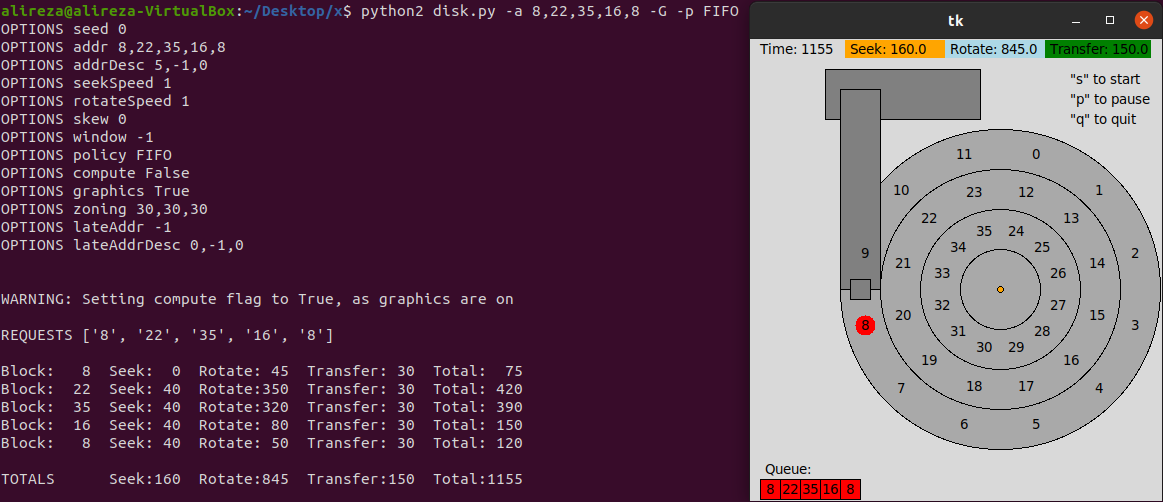
\includegraphics[width=1\textwidth]{figures/6-a.png}
    \caption
	{
\lr{FCFS}
	}
    \label{fig:fig1}
\end{figure}
\begin{figure}[H]
    \centering
    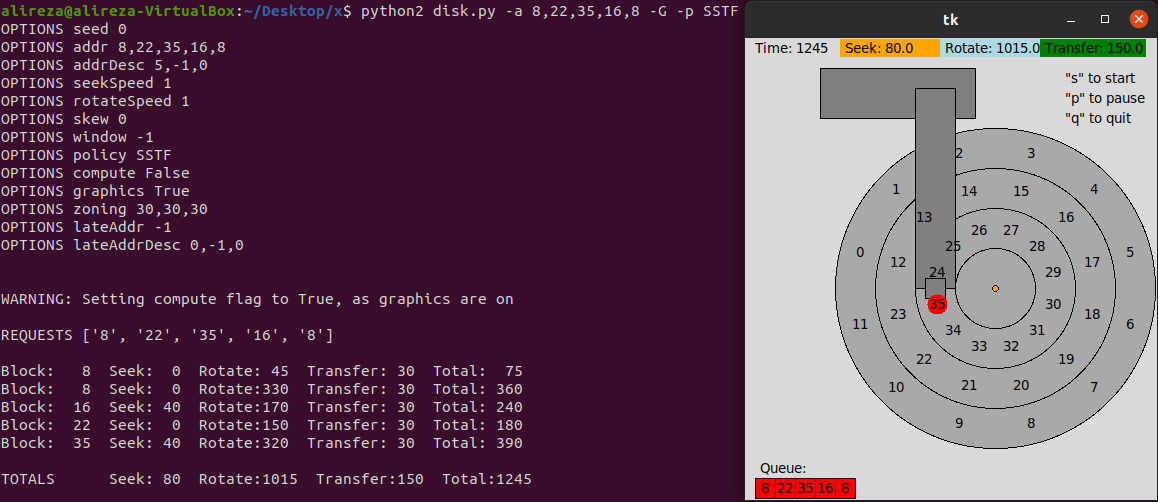
\includegraphics[width=1\textwidth]{figures/6-b.png}
    \caption
	{
\lr{SSTF}
	}
    \label{fig:fig1}
\end{figure}
برای ورودی مذکور الگوریتم \lr{FCFS} در 1185 واحد و الگوریتم \lr{SSTF} در 1245 واحد زمانی اجرا می‌شود. در این مجموعه از ورودی‌ها چون \lr{distance}ِ دو بلاک برای \lr{Rotate} کم است ولی \lr{distance}ِ \lr{seek} زیاد است.



\section*{منابع}
\renewcommand{\section}[2]{}%
\begin{thebibliography}{99} % assumes less than 100 references
%چنانچه مرجع فارسی نیز داشته باشید باید دستور فوق را فعال کنید و مراجع فارسی خود را بعد از این دستور وارد کنید


\begin{LTRitems}

\resetlatinfont

\bibitem{b1}

\end{LTRitems}

\end{thebibliography}


\end{document}
